\documentclass[hidelinks, 12pt, oneside]{article}
\usepackage{bookmark}
\usepackage{graphicx}
\usepackage{hyperref}
\usepackage{titlesec}
\setcounter{secnumdepth}{4}
\usepackage[utf8]{inputenc}
\usepackage[english]{babel}
\usepackage{color}


\begin{document}

	\begin{center}
    \centering
    
%University logo
    
\includegraphics[width=144px]{img/icon.png}
    \rule{0\linewidth}{0.15\linewidth}\par
    
    		\begin{center}
		{\uppercase{\Large User Manual\par}}
   		{\Large iCrawler \par}
   			\vspace{1cm} 
   		{\Large Emilio Mumba  \par} 
    		\vspace{1cm}
		   		
    		{\Large The 5 Concurrent Nodes \par} 
    		\vspace{1cm}
		
		{\normalsize Khathutshelo Shaun Matidza\par}
		{\normalsize Sylvester Sandile Mpangane\par}
		{\normalsize Thabang Michael Letageng\par}
		{\normalsize Matthew Nel\par}
		
		\end{center}

		\textbf{}		
		\centering
		\vspace{2cm}
		Department of Computer Science, University of Pretoria

		
	 	{\Large  September 2015}
\end{center}
\clearpage


	\tableofcontents
	\newpage
	
	\section{Overview}
	\emph{iCrawler} is a mobile device monitoring app available for Android only. The objective of the app is to display and assist in understanding the activities performed by a mobile user as well as shedding more light into the behaviour of the mobile user. The mobile monitoring application generates reports giving the investigator quick and comprehensive data/logs. The app
uses the device's internet connection to send the data logs collected from the device to a desktop-dashboard for review. The app is absolutely free to download.\newline\newline
	 
	 \uppercase{Why use the \MakeLowercase iCrawler App:}\newline
	 \begin{itemize}
		\item Child monitoring\newline
		\emph{iCrawler} can be used by parents/guardians to monitor activities that their minor
		 children get up to.	
		\item Employee monitoring\newline
		Companies that hand out mobile devices to their employees can use the \emph{iCrawler} app to monitor any 
		unauthorized activities that employees might be getting up to.
	\end{itemize}
	\newpage
	
	
	\section{Configuration}
	
	\begin{tabular}{ |l|l| }  \multicolumn{2}{|c|}{
\includegraphics[width=0.1 \textwidth]{img/icon.png}iCrawler}
	 \\ \hline\noalign{\smallskip} \textbf{Stable release} & 1.0
	  \\\\ \noalign{\smallskip} \textbf{Development status}& Active
	  \\\\ \noalign{\smallskip}\textbf{Operating System}& Android 4.2+
	  \\\\ \noalign{\smallskip}\textbf{Platform}& Android
	  \\\\ \noalign{\smallskip}\textbf{Internet connection} & Yes
	  \\\\ \noalign{\smallskip}\textbf{Available in} & English
	  \\\\ \noalign{\smallskip}\textbf{Type}& Monitoring Application
	  \\\\ \noalign{\smallskip}\textbf{License}& Free
	  \\\\ \noalign{\smallskip}\textbf{Website}& www.github.com/u11241617/COS301-Mobile-Monitoring-App
	  %\hline
	 \end{tabular}\newpage
	%%%%%%%%%%%%%%%%%%%%%%%%%%%%%%%%%%%%%%%%%%%%%%%%%%%%%%%%%%%%%%%%%%%%%%%%%%%%%%%%%%%
	\section{User Access Levels}
		Our Github repository is private, only invited users can download the appliaction, additionaly a user has  to be registered on iCrawler to be able to have the app submit their user activities onto the dashboard, and to be able to log onto the dashboard.\newline
	\section{Installation}
	The iCrawler APK (Android Application Kit) is currently only available for download on our GitHub repository. Follow this link inorder 
	to start the download\dots\newline
		\href{url}{https://github.com/u11241617/COS301-Mobile-Monitoring-App/tree/master\\/Android\%20Project/}\\
		\emph{NB:} Open the \emph{app-release} folder to find the apk \newline \newline
		When the download has successfully completed the installation should automatically start, if not follow the following steps:\newline
	  
	 \begin{enumerate}
 	 	\item Navigate to 'File Management' from the options menu on your device
 	 	\item Under 'Device Storage', locate a folder named 'Download'
 	 	\item Locate and launch a file named 'iCrawler.apk' within this folder
 	 	\item When a 'Install blocked' popup appears, select the 'Settings' option
 	 	\item Scroll down and check the option 'Unknown Sources'
 	 	\item Another popup will appear, simply click 'OK' then 'Next' followed by 'Install'
 	 	\item On completion you will see the options 'Done' and 'Open', click 'Open' to start the app \ldots
 	\end{enumerate}\newpage


	\section{Getting Started}
	After successful installation, locate the iCrawler app icon and click on it to run the app.
	 \begin{itemize}
	 	\item \textbf{Terms and Conditions}\newline
	 	Before you can use iCrawler you neeed to read the 'Terms and Conditions' on startup and only 
	 	after accepting them can you proceed, if you don't accept you can not use the app.
	 	 
	 	 %terms and conditions screenshot here%
	 	 \begin{figure}[h!]
	 	 	\caption{Terms and Conditions page}
	 	 	\centering 																												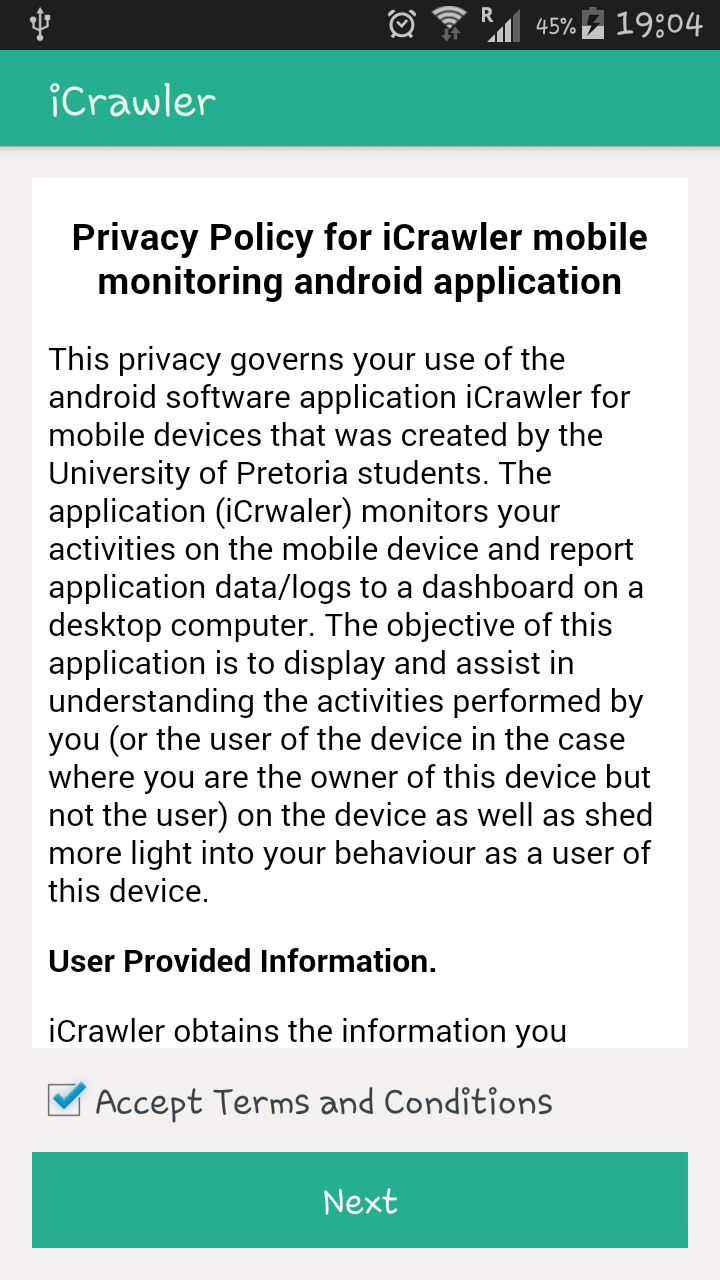
\includegraphics[width=0.5 \textwidth]{img/tnc2.png}
	 	 \end{figure}\newpage
	 	 
	 	\item \textbf{Sign up new user}\newline
	 	If you are a first time user you need to sign up after accepting the 'Terms and Conditions'. You need
	 	to provide a working \emph{email address} and create a \emph{password} you will use to sign in with in future.
	 	If you have an existing account, simply 'click Sign in' to go to the sign in page.
	 	 
	 	 %register new user screenshot here%
	 	 \begin{figure}[h!]
	 	 	\caption{Sign up user page}
	 	 	\centering 																												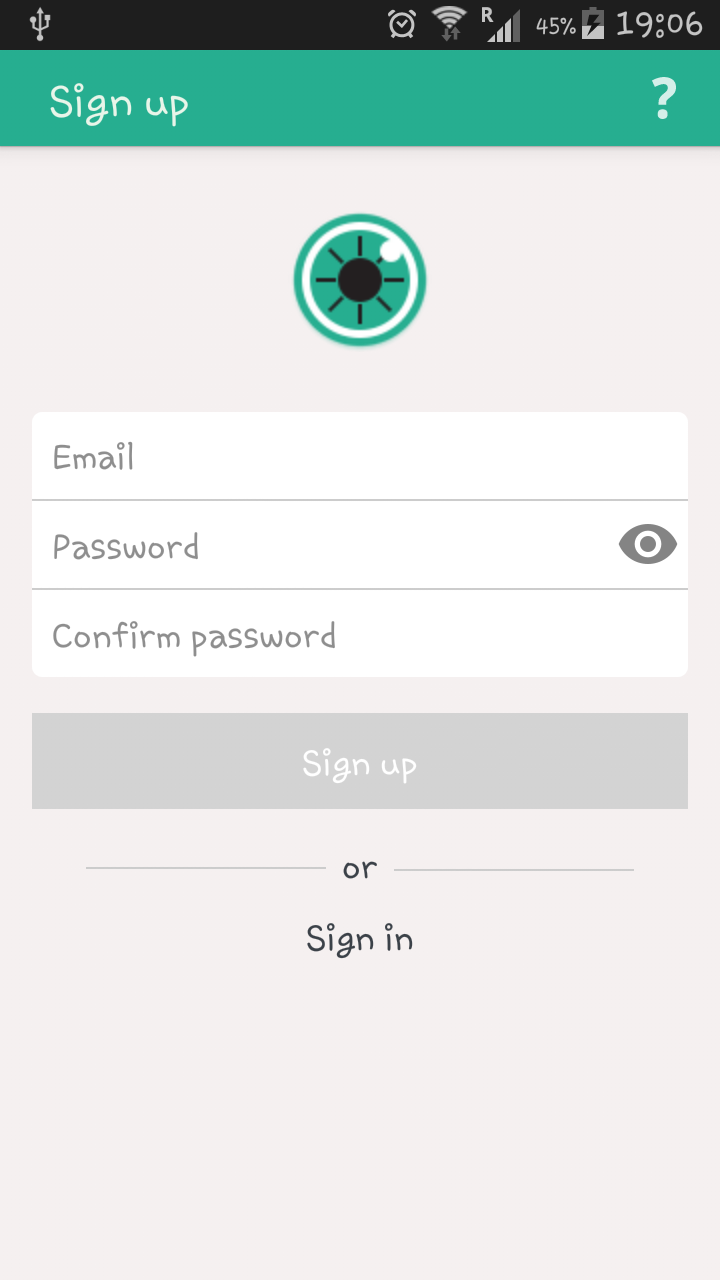
\includegraphics[width=0.5 \textwidth]{img/reg.png}
	 	 \end{figure}\newpage
	 	 
	 	\item \textbf{Sign in as existing user}\newline
	 	If you have used the iCrawler app before, you need not to sign up again, simply enter your credentials and then
	 	'click Sign in' in order to subscribe the new device. If not, 'click Sign up' to register as a new user.
	 	
	 	%login user screenshot here%
	 	 \begin{figure}[h!]
	 	 	\caption{Sign in user page}
	 	 	\centering 																												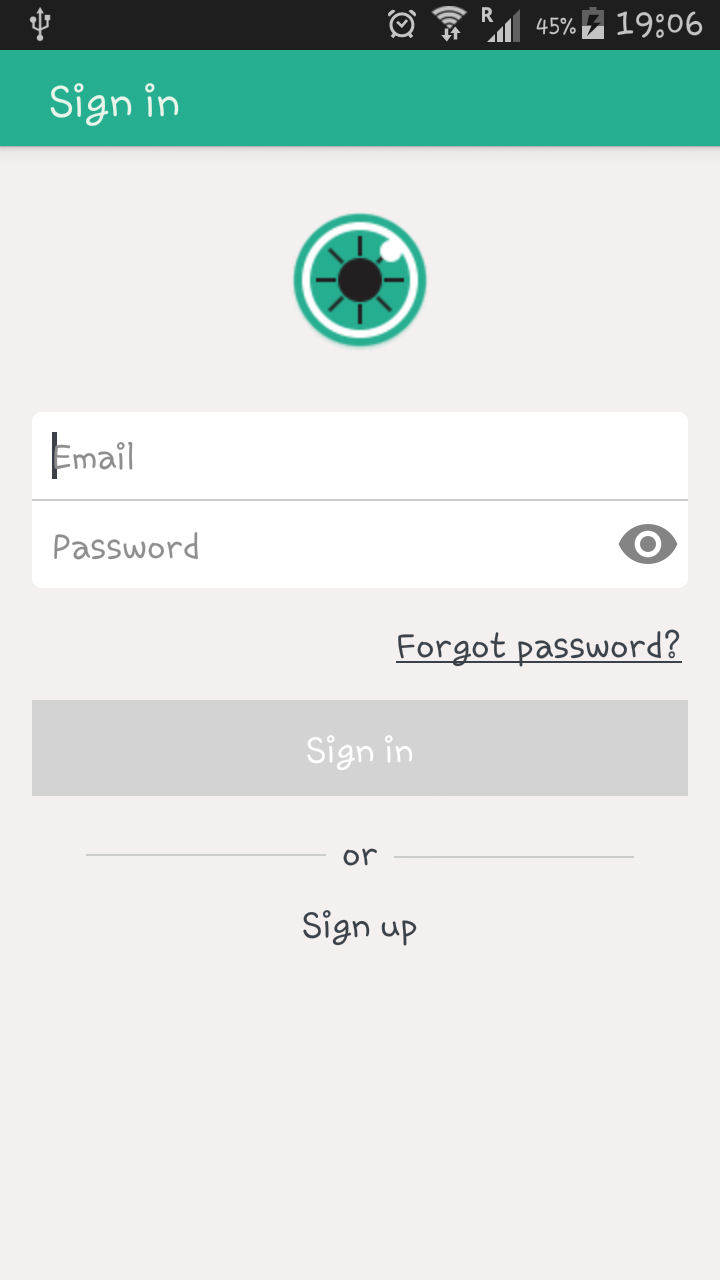
\includegraphics[width=0.5 \textwidth]{img/log.png}
	 	 \end{figure}
	 	 
	 \end{itemize}\newpage
	 
	 
	\section{Using the App}
	The app runs in the background after 'Signing up or Signing in'; there is no other form of interaction with 
	the app thereafter. You can access the log reports generated via the dashboard.
	\newline\newline
	
	\section{Troubleshooting}
	The following section lists some of the iCrawler app's possible issues and resolutions:
	
	\begin{itemize}
		\item \textbf{Does not launch.} Restart your phone and try to launch the application again.
		\item\textbf{Crashes immediately after launch.} Ensure that your device meets the minimum specifications to run
		 iCrawler (See configurations). Go to Settings $\rightarrow$ Apps $\rightarrow$ Manage Apps $\rightarrow$ Running, to check if your apps are not using up all
		  your memory. Try to end all processes you do not need and re-start your phone.
		\item \textbf{Other unknown causes.} If problems continue, delete the app completely and then reinstall it from Google Play Store.\
	\end{itemize}
		
\end{document}
